\chapter{Introduction}\label{ch:introduction}

\epigraph{\normalsize\textit{ "What I cannot create, I do not understand."}}{\normalsize\textit{ Richard Feynman}}

One of the main aspirations of Artificial Intelligence is to develop algorithms and techniques that enrich computers with ability to understand our world. Generative models are one of the most promising approaches towards achieving this goal.\par\bigskip


\section{Generative Models}
\label{sec:gm}
A generative model is a mathematical or statistical model to generate all values of a phenomena. To train such a model, we first collect a large amount of data in some domain (e.g., think millions of images, sentences, or sounds, etc.) and then train a model to generate data like it.\par\bigskip
A generative algorithm models how data was generated to classify a data instance. It poses the question: according to my generation hypotheses, which category is most likely to generate this data instance? A discriminative algorithm does not care about how the data was generated, it just classifies a given data instance; that is, given the features of a data instance, they predict a label or category to which that data belong. Discriminative models learn the boundary between classes while Generative models model the distribution of individual classes; that is, a generative model learns the joint probability distribution $p(x,y)$ while a discriminative model learns the conditional probability distribution $p(y|x)$ “probability of y given x”.\par\bigskip
The trick is that the neural networks that we use as generating models have a significantly smaller number of parameters than the amount of data on which we train them, so the models are forced to effectively discover and internalize the essence of the data to generate it.\par\bigskip
\noindent There are multiple approaches to build a generative models
  \subsection{Generative adversarial networks}
  \label{sub:gans}
  Generative adversarial networks (GANs) are a class of generative algorithms used in unsupervised machine learning, implemented by a system of two neural networks competing in a zero-sum game framework. They were presented by Ian Goodfellow \textit{et al}. \cite{gan}. This technique can generate photographs that seem at least superficially authentic to human observers, having many realistic features (though in tests people can tell real from generated in some cases).
  \subsection{Variational Autoencoders } 
  \label{sub:vae}
  An autoencoder network is actually a pair of two connected networks, an encoder and a decoder. An encoder network receives an input and converts it into a smaller, denser representation that the decoder network can use to convert it back to the original input. Variational Autoencoders (VAEs) have one fundamentally unique property that separates them from vanilla autoencoders, and it is this property that makes them so useful for generative modeling: their latent spaces are, by design, continuous, allowing easy random sampling and interpolation. Variational Autoencoders (VAEs) allow us to formalize generative modeling problem in the framework of probabilistic graphical models where we are maximizing a lower bound on the log likelihood of the data
  \subsection{Autoregressive models} 
  \label{sub:autoregressive} 
  Autoregressive models such as PixelRNN, on the other hand train a network that models the conditional distribution of every individual pixel given previous pixels (to the left and to the top). These models efficiently generate independent,exact samples via ancestral sampling. This is similar to plugging the pixels of the image into a char-rnn, but the RNNs runs both horizontally and vertically over the image instead of just a 1D sequence of characters.\par\bigskip

\section{Generative Adversarial Networks} % (fold)
\label{sec:generative_adversarial_networks}
\begin{figure}[H]
\centering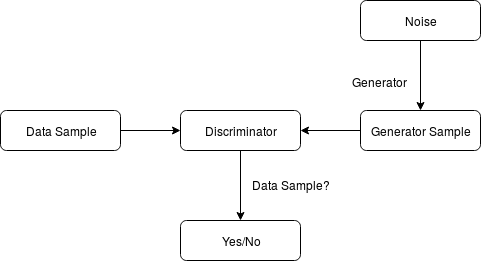
\includegraphics[width=.7\textwidth]{images/vanillaGAN.png}
\caption{Vanilla Generative Adversarial Network}
\label{fig:gans}
\end{figure}
Generative Adversarial Networks, which we already discussed above, pose the training process as a game between two distinct networks: A neural network, called the generator, generates new instances of data, while the other, the discriminator, evaluates their authenticity; discriminator network tries to classify samples as either coming from the true distribution $p(x)$ or the model distribution $\hat{p}(x)$. Every time the discriminator notices a difference between the two distributions the generator adjusts its parameters slightly to make it go away, until at the end (in theory) the generator exactly reproduces the true data distribution and the discriminator is guessing at random, unable to find a difference.\par\bigskip
The generator takes noise as input and attempts to produce an image that belongs to the real distribution; that is, it tries to fool the discriminator to accept it as real image. Discriminator takes a generated image or a real image as input and attempts to correctly classify the image as real or fake (generated).\par\bigskip
To learn the distribution of the generator $p_g$ over data $\bm{x}$, we define a prior on input noise variables $p_{\bm{z}}(\bm{z})$, then represent a mapping to data space as $G(\bm{z}; \theta_g)$, where $G$ is a differentiable function represented by a neural network with parameters $\theta_g$. We define a second neural network $D(\bm{x}; \theta_d)$ that outputs a single scalar. $D(\bm{x})$ represents the probability that $\bm{x}$ came from the data rather than $p_g$. We train $D$ to maximize the probability of assigning the correct label to the training examples and samples of $G$. We simultaneously train $G$ to minimize $\log(1-D(G(\bm{z})))$.\par\bigskip
\noindent This can be represented minimax game \\
\begin{equation} \label{eu_eqn}
\min_{G} \max_{D} V(D, G)=\mathbb{E}_{\bm{x} \sim p_{\text{data}}(\bm{x})}[\log D(\bm{x})]+\mathbb{E}_{\bm{z} \sim p_{\bm{z}}(\bm{z})}[\log (1 - D(G(\bm{z})))]
\end{equation}
% section generative_adversarial_networks (end)

\section{Convolutional Neural Networks} % (fold)
\label{sec:convolutional_neural_networks}

\begin{figure}[H]
\centering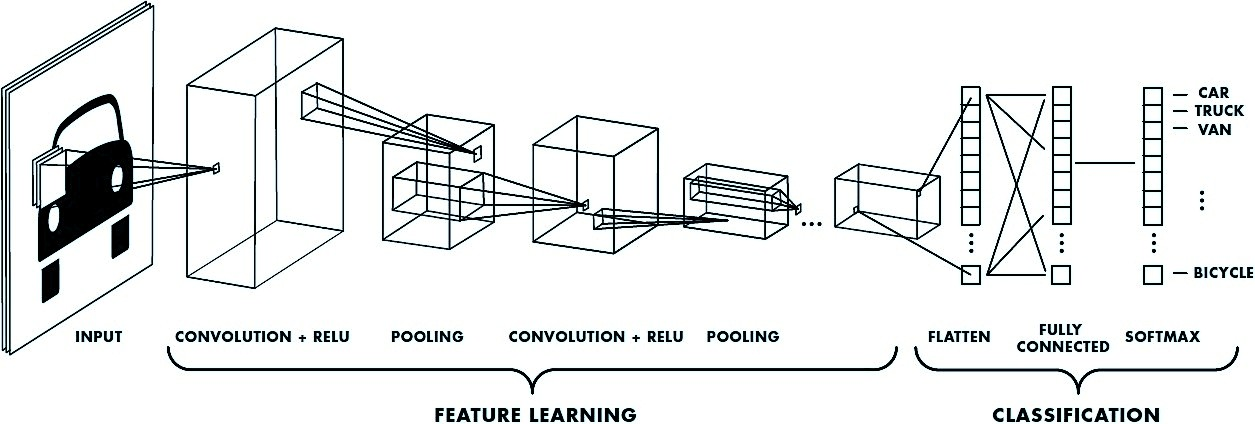
\includegraphics[width=.7\textwidth]{images/CNN.jpg}
\caption{Convolutional Neural Network}
\label{fig:cnn}
\end{figure}
Before we can jump to understanding Capsule Networks, we need to know about Convolutional Neural Networks(CNNs). Convolutional neural networks are very similar to ordinary neural networks, they consist of neurons that have learn-able weights and biases. Each neuron receives inputs, performs a scalar product and possibly follows it with a nonlinearity. The entire network expresses a single differentiable score function: raw image pixels at one end to class scores at the other end. And they still have a loss function on the last layer.\par\bigskip
The major difference is that CNN explicitly assumes that the inputs are images, which allows us to encode certain properties in the architecture. These then make the forward functions more efficient to implement and significantly reduces the amount of parameters in the network.\par\bigskip
Ordinary neural networks don’t scale well to full images, for example, A colour image of dimensions of 150x150 (which is considered as low resolution by most people) has a shape (150,150,3), a fully connected neuron on first layer which receives this image would require 67500 weights. Unlike an ordinary neural network, the layers of a CNN have neurons arranged in 3 dimensions: width, height, depth as shown in figure \ref{fig:cnn}. The neurons in a layer will only be connected to a small region of the layer before it, instead of all of the neurons in a fully-connected manner. CNN  will reduce the full image into a single vector of class scores, arranged along the depth dimension.\par\bigskip
CNNs use a "Pooling" layer to reduce the spatial size of the input for each convolutional layer. The Pooling Layer operates independently on every depth slice of the input and resizes it spatially, generally using the MAX operation, hence pooling layer is sometimes referred to as Max Pooling layer.
% section convolutional_neural_network (end)

\section{Capsule Networks} % (fold)
\label{sec:capsule_networks}
“The pooling operation used in convolutional neural networks is a big mistake and the fact that it works so well is a disaster.” says Geoffrey Hinton, one of the founders of deep learning (Also known as Godfather of Deep Learning) and an inventor of numerous models and algorithms that are widely used today. CNNs perform exceptionally great when they are classifying images which are very close to the data set. If the images have rotation, tilt or any other different orientation then CNNs have poor performance. This problem is usually partially solved by adding different variations of the same image during training. But CNNs still require large amount of data to perform reasonably well. We use pooling after each layer to make it compute in reasonable time frames. But in essence, it also loses out the positional data.\par\bigskip
\begin{figure}[H]
\centering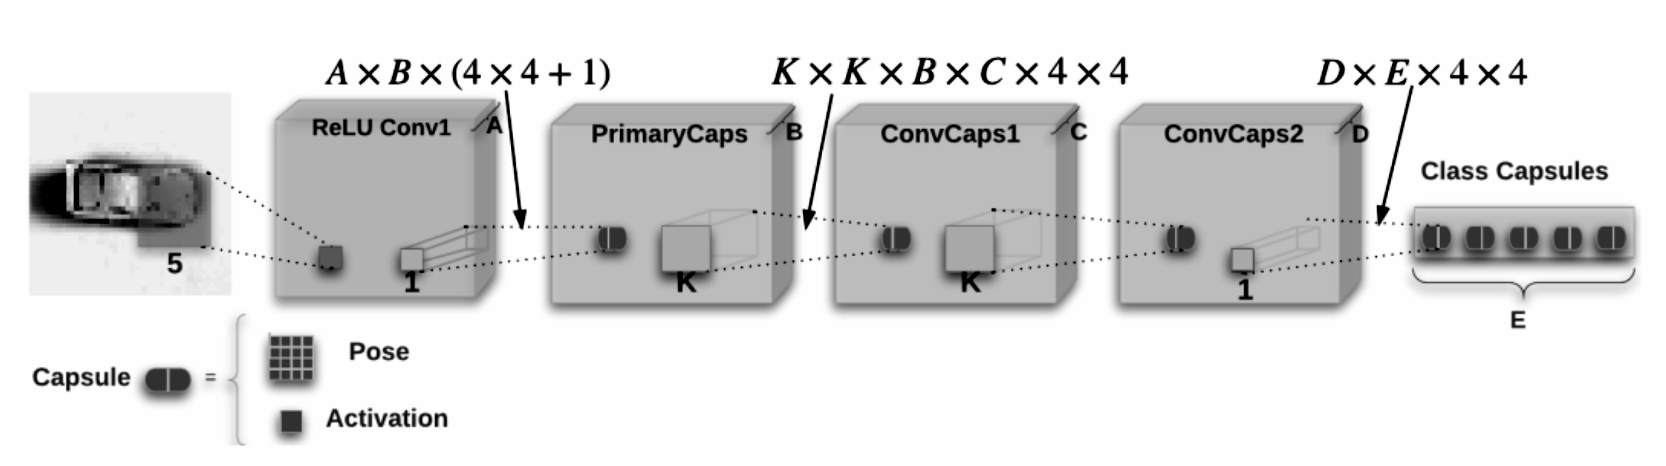
\includegraphics[width=.7\textwidth]{images/caps.png}
\caption{Capsule Networks}
\label{fig:caps}
\end{figure}
What we need is not invariance but equivariance. Invariance makes a CNN tolerant to small changes in the viewpoint. Equivariance makes a CNN understand the rotation or proportion change and adapt itself accordingly so that the spatial positioning inside an image is not lost. This leads us to Capsule Networks.\par\bigskip
Capsule is a nested set of neural layers as shown in figure \ref{fig:caps}. Capsules are like cortical columns in human brains. Deep neural nets learn by back-propagation of errors over the entire network. In contrast real brains supposedly wire neurons by Hebbian principles: “units that fire together, wire together”. Capsules mimic Hebbian learning in the way that: “A lower-level capsule prefers to send its output to higher level capsules whose activity vectors have a big scalar product with the prediction coming from the lower-level capsule”. Capsules, combination of capsules encodes objects parts AND their relative positions, so an object instance can be accurately derived from the presence of the parts at the right locations, and not just their presence. Capsules produce equivariant features. Capsules predict the activity of higher-layer capsules to route information to right higher-layer capsules, this is called "Dynamic routing".
% section capsule_networks (end)

\section{Semantic Inpainting} % (fold)
\label{sec:semantic_inpainting}
To demonstrate the application of our modified GAN, we will be using Semantic Inpainting. Inpainting is the process of reconstructing lost or deteriorated parts of images and videos. In the museum world, in the case of a valuable painting, this task would be carried out by a skilled art conservator or art restorer. In the digital world, inpainting (also known as image interpolation or video interpolation) refers to the application of sophisticated algorithms to replace lost or corrupted parts of the image data (mainly small regions or to remove small defects). Here we will be using GAN to implement semantic inpainting.
% section semantic_in_painting (end)

\section{Scope of work} % (fold)
\label{sec:scope_of_work}
Generative Adversarial Networks are one of the hottest topics in Deep Learning right now. The applications of GANs are far ranging and immense. Creating Info-graphics from text, creating animations for rapid development of marketing content, generating website designs are to name a few. Our focus in this project is to implement a way to complete images of faces by generating the missing pieces using a GAN. 

\par\bigskip
This particular implementation of the technology would be immensely useful in a variety of circumstances. A few straightforward applications include face sketching of suspects in a crime using eye witness accounts, super resolution of CCTV camera footage to enhance faces, filling in of old degraded color photos, etc.
% section scope_of_work (end)

\section{Motivation} % (fold)
\label{sec:motivation}
The existing latest state-of-the-art GAN architectures use Convolution Neural Networks in their Generators and Discriminators. The CNNs are said to have the drawbacks as mentioned before, where they cannot understand orientation and spatial relationships unless they are extensively trained with all possible images. This major drawback is handled by Capsule Networks.\par\bigskip
Using the CapsNet architecture into the Generator/Discriminator could improve these Adversarial Networks quite drastically. This mating of the revolutionary Generative Adversarial Networks along with the ground-breaking Capsule Networks, resulting in “Capsule Net GANs” is the overarching objective.
% section motivation (end)